\documentclass[12pt]{beamer}
\usepackage[utf8]{inputenc}
\usepackage[T1]{fontenc}
\usepackage[spanish]{babel}
\usepackage{xcolor}
\usepackage{tcolorbox}
\usepackage{amsthm}
\usepackage{amsmath}
\usepackage{lipsum}
\usepackage{tikz}
\usepackage{lmodern}
\usepackage{graphicx}
\usepackage[boxed,algoruled,linesnumbered]{algorithm2e}
\renewcommand{\familydefault}{\sfdefault}


% Configuración de algorithm2e para Beamer
\SetAlgoNlRelativeSize{-1}
\SetNlSty{textbf}{(}{)}
\SetAlFnt{\small}
\SetInd{0.5em}{0.5em} % Ajusta la indentación
\SetAlCapSkip{1em}

% ====== DEFINICIÓN DE COLORES ======
\definecolor{rojoUNI}{HTML}{D16969}
\definecolor{doradoUNI}{HTML}{DBCB9F}
\definecolor{rojoSuave}{HTML}{d39c9c}
\definecolor{doradoClaro}{HTML}{eee5cd}
\definecolor{grisNeutro}{HTML}{9B9B9B}

% ====== CONFIGURACIÓN BEAMER ======
%\usetheme{Madrid}
%\usecolortheme{default}

% Personalización de colores de Beamer
\setbeamercolor{title}{fg=rojoUNI}
\setbeamercolor{frametitle}{fg=rojoUNI}
\setbeamercolor{structure}{fg=rojoUNI}
\setbeamercolor{normal text}{fg=black}
\setbeamercolor{block title}{fg=white, bg=rojoUNI}
\setbeamercolor{block body}{fg=black, bg=doradoClaro!40}

% Pie de página personalizado
\setbeamertemplate{footline}{
  \begin{tikzpicture}[remember picture,overlay]
    \node at (current page.south) [anchor=south, yshift=0.6cm] {
      
\includegraphics[width=0.85\paperwidth,height=0.8cm]{img/footage-red.pdf}
    };
  \end{tikzpicture}
  \hspace*{0.1\paperwidth}
  \raisebox{0.5cm}[0pt][0pt]{
    \color{rojoUNI}\bfseries\insertshorttitle
  }
  \hfill
  \raisebox{0.5cm}[0pt][0pt]{
    \color{rojoUNI}\bfseries\insertframenumber/\inserttotalframenumber
  }
  \hspace*{0.1\paperwidth}
}

% Configuración de bloques
\newtcolorbox{definicion}[1][]{colback=doradoClaro!40,
  colframe=rojoUNI, fonttitle=\bfseries\color{white},
  title=Definición, #1}

\newtcolorbox{teorema}[1][]{colback=white,
  colframe=doradoUNI, fonttitle=\bfseries\color{black},
  title=Teorema, #1}

\newtcolorbox{lema}[1][]{colback=white,
  colframe=rojoSuave, fonttitle=\bfseries\color{white},
  title=Lema, #1}

\newtcolorbox{ejemplo}[1][]{colback=white,
  colframe=rojoSuave!80!black, fonttitle=\bfseries\color{white},
  title=Ejemplo, #1}

\newtcolorbox{restriccion}[1][]{colback=doradoClaro,
  colframe=grisNeutro, fonttitle=\bfseries\color{white},
  title=Restricción, #1}

\newtcolorbox{restriccionesPC}[1][]{colback=doradoClaro!40,
  colframe=rojoUNI, fonttitle=\bfseries\color{white},
  title=Restricciones, #1}

\newtcolorbox{bloque}[1][]{
  colback=doradoClaro!40,
  colframe=rojoUNI,
  fonttitle=\bfseries\color{white},
  title=#1}

% ====== DOCUMENTO ======
\title{Greedy para zebras}
\author{Miguel Miní}
\date{2025}

\begin{document}

\begin{frame}

  {\hspace{9cm}
\includegraphics[width=0.15\textwidth]{img/unicamp.png}}
  
  %\vspace{-0.5cm}
  
  % Título
  
  {\hspace{0.5cm}\bfseries\Huge \textcolor{rojoUNI}{Greedy para zebras}}

   \vspace{0.5cm}
  {\hspace{0.6cm}\textcolor{rojoUNI}{Miguel Miní}}
  
  \vfill
\end{frame}


\begin{frame}{Huffman Tree}

\begin{definicion}
    El Huffman Tree de una secuencia $\{w_1, w_2, \dots, w_n\}$ es un árbol binario con $n$ hojas, tal que minimiza

\[
    \sum_{i=1}^n w_i \times d_i  
\]

    Donde $d_i$ ($1 \le i \le n$), es la profundidad de la i-ésima hoja en el árbol.
\end{definicion}
  
\end{frame}

\begin{frame}

\begin{ejemplo}
\begin{columns}
\begin{column}{0.6\textwidth}
Huffman Tree con costo 
\begin{align*}
    &w_1 \times 2 + w_2 \times 2 + w_3 \times 1\\
    &2 \times 2 + 3 \times 2 + 6 \times 1 = 16
\end{align*}

\textbf{Nota:} Tambien podemos comprimir frases usando el camino hacia cada letra (izquieda: 0, derecha: 1).
    
\end{column}

\begin{column}{0.31\textwidth}
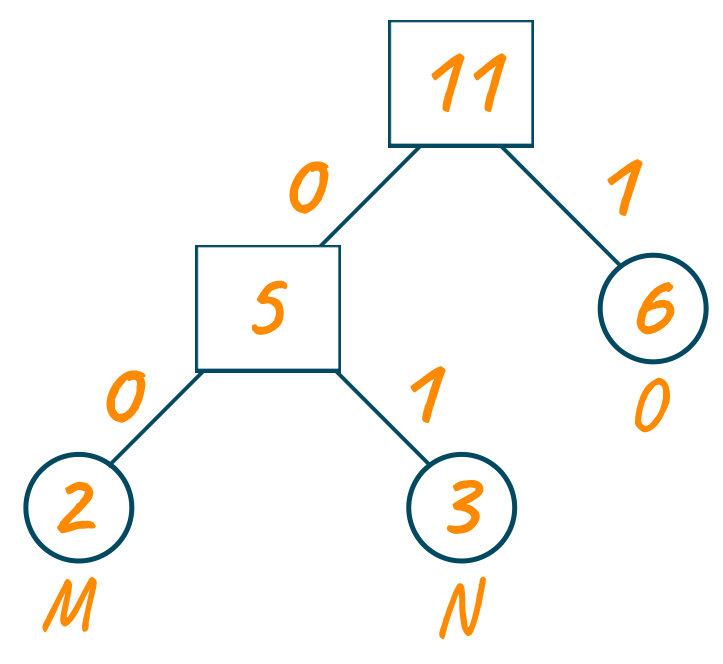
\includegraphics[width=\textwidth]{img/huffman.png}    
\end{column}

\end{columns}
\end{ejemplo}

\end{frame}

\begin{frame}
\hspace*{0.5cm} % Ajuste para mover el algoritmo a la derecha
\begin{minipage}{0.9\textwidth}
\SetAlFnt{\footnotesize} % Reducir tamaño de fuente
\begin{algorithm}[H]
  \KwIn{secuencia $w_1, w_2, \dots, w_n$}
  \KwOut{Huffman Tree}
  min heap $Q$ con todas las hojas ($nodo_i, w_i$), ordenados por $w_i$\;
  \While{$|Q| > 1$}{
      $(node_i, w_i)\leftarrow$ extraer top de $Q$\;
      $(node_j, w_j) \leftarrow$ extraer top de $Q$\;
      Crear un nuevo nodo $node_z$ con hijos $node_i$ y $node_j$\;
      Asignar $w_z = w_i + w_j$\;
      Insertar $(node_z, w_z)$ en la cola $Q$\;
  }
  \Return{El único nodo restante en $Q$ (raíz del árbol)}
  \caption{Construcción de un Huffman Tree}
\end{algorithm}
\end{minipage}
\end{frame}

\begin{frame}
\begin{ejemplo}
\begin{figure}
    \centering
    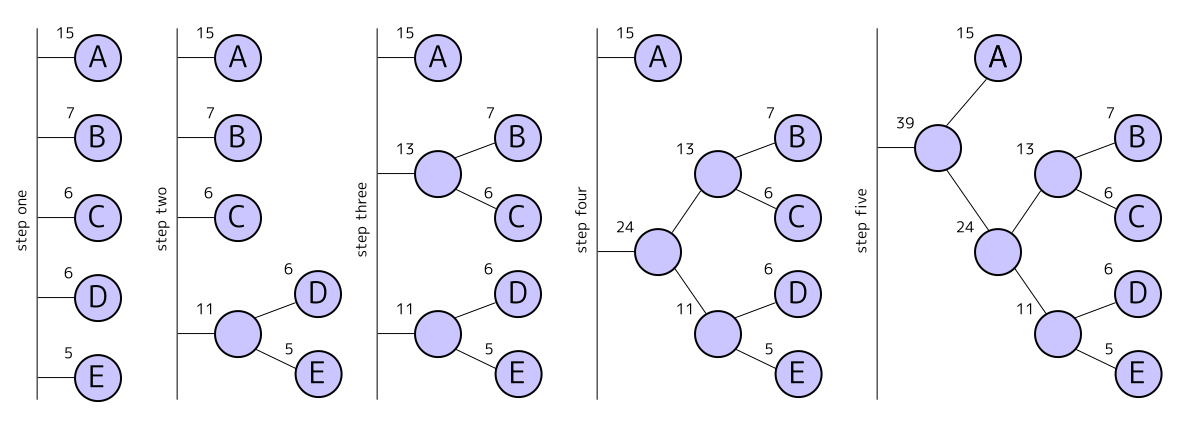
\includegraphics[width=1\linewidth]{img/huffmanalgorithm.png}
    \label{fig:enter-label}
\end{figure}  
\end{ejemplo}    
\end{frame}

\begin{frame}
\begin{bloque}[Revisitando Huffman Tree]
Dado que el algoritmo es óptimo*, podemos concluir que este tiene un costo inferior a alguna configuración, así:

\[
\sum_{i=1}^n w_i \times d_i \le \left(\sum_{i=1}^n w_i\right) \log (n)
\]

\pause

\textbf{hint:}

\begin{figure}
    \centering
    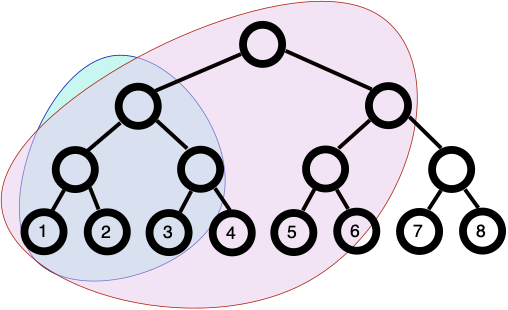
\includegraphics[width=0.4\linewidth, height=0.23\textwidth]{img/complete.png}
    \label{fig:enter-label}
\end{figure}

\end{bloque}
\end{frame}

\begin{frame}
\begin{bloque}[Revisitando Huffman Tree]

Sean $n$ conjuntos con pesos $\{w_1, w_2, \dots, w_n\}$, y debemos formar un conjunto que contenga a todos ellos, tal que:

\begin{itemize}
    \item escogemos dos conjuntos $s_x$ y $s_y$.
    \item creamos un nuevo conjunto $s_z = s_x \cup s_y$, con costo $w_z = w_x + w_y$.
    \item reemplazamos $s_x$ y $s_y$ con $s_z$.
\end{itemize}

Deseamos que la suma de costos sea mínima.

\end{bloque}
\end{frame}

\begin{frame}
\begin{bloque}[Revisitando Huffman Tree]
¿El problema es equivalente a hallar un Huffman Tree?

\begin{columns}
\begin{column}{0.4\textwidth}
\begin{figure}
    \centering
    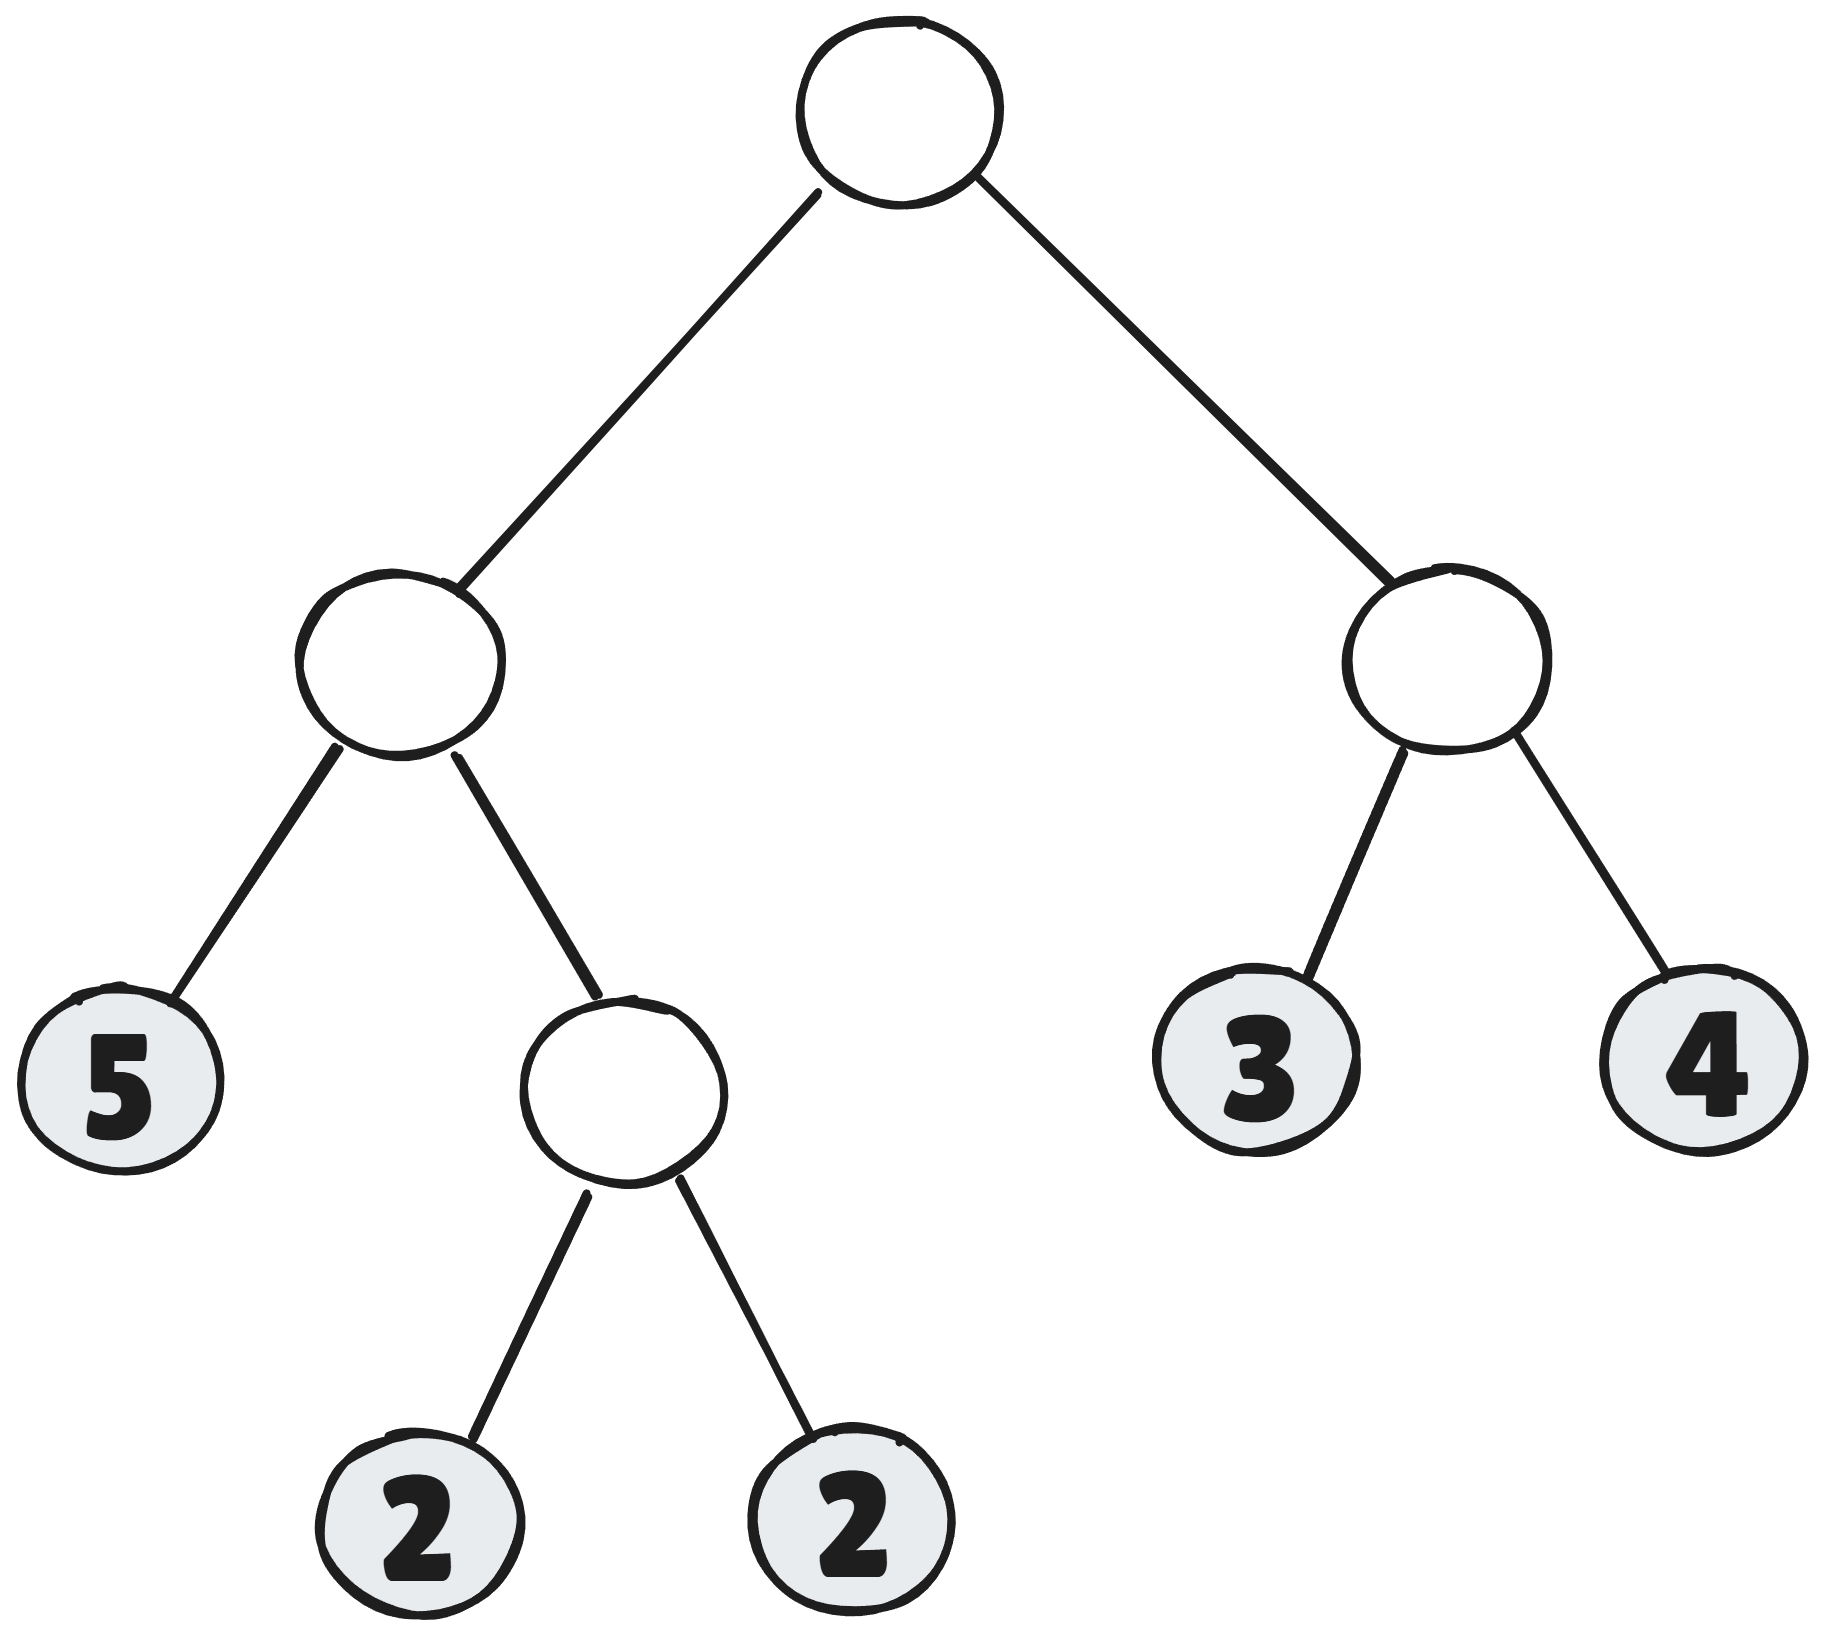
\includegraphics[width=\linewidth]{img/ht1.png}
    \label{fig:enter-label}
\end{figure}
\end{column}
\begin{column}{0.4\textwidth}
\begin{figure}
    \centering
    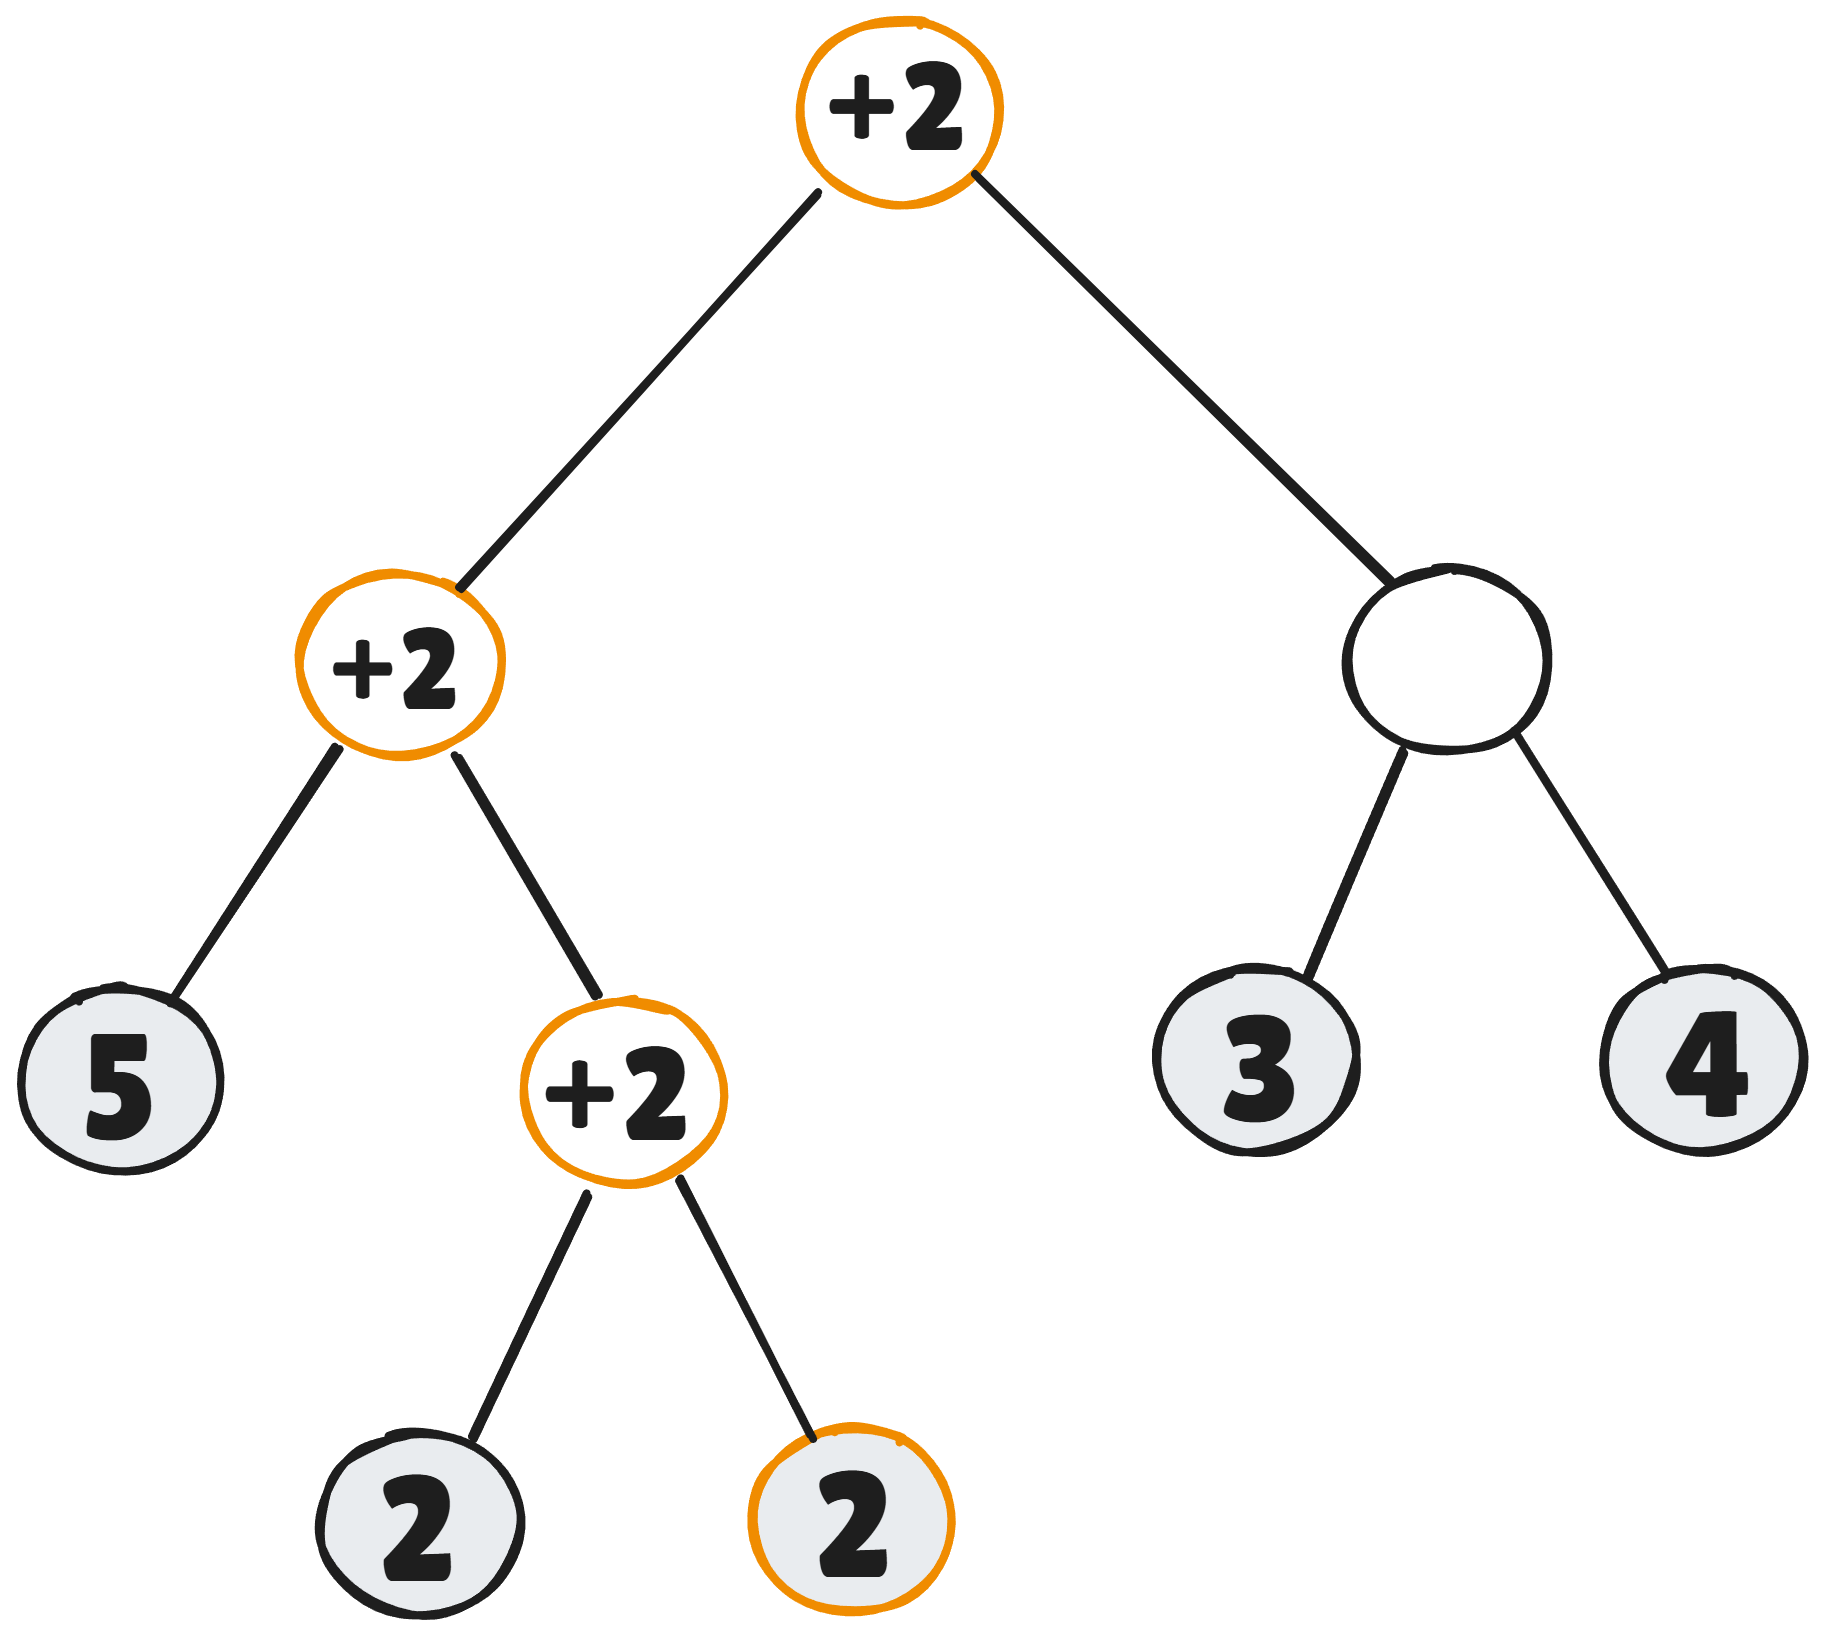
\includegraphics[width=\linewidth]{img/ht2.png}
    \label{fig:enter-label}
\end{figure}
\end{column}
\end{columns}
\end{bloque}
\end{frame}

\begin{frame}
\begin{bloque}[Revisitando Huffman Tree]
¿El problema es equivalente a hallar un Huffman Tree?

\begin{figure}
    \centering
    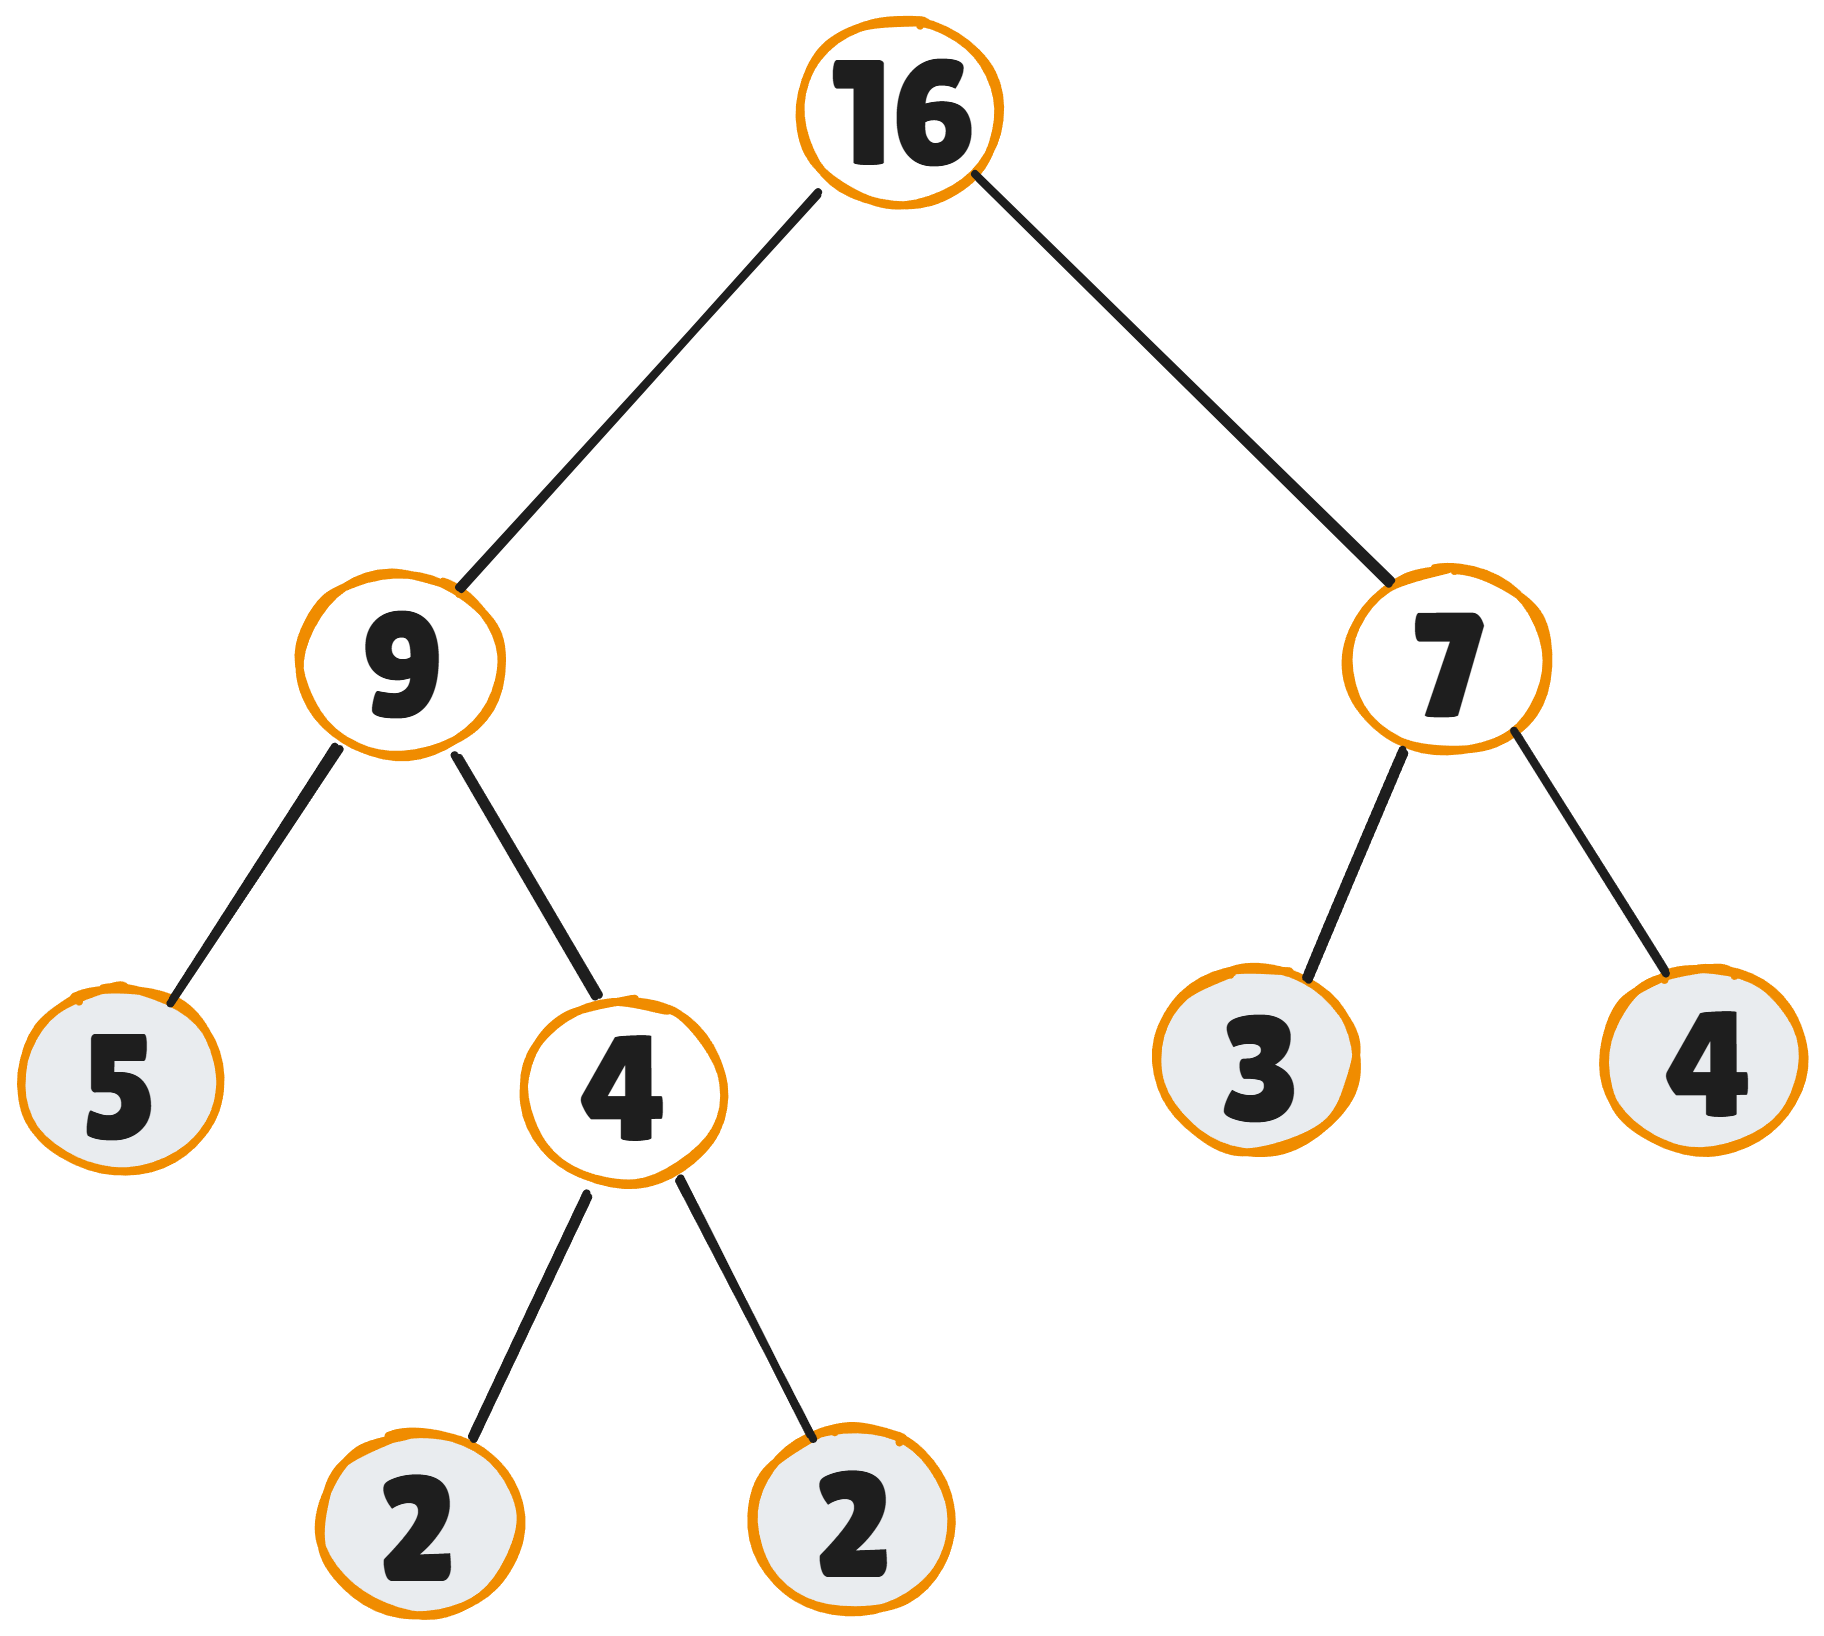
\includegraphics[width=0.4\linewidth]{img/ht3.png}
    \label{fig:enter-label}
\end{figure}

\end{bloque}
\end{frame}

\begin{frame}
\begin{bloque}[Revisitando Huffman Tree]

\begin{itemize}
    \item Por tanto, el algoritmo de Huffman Tree genera un costo optimo para el problema. 
    \pause
    \item Aplicación: Deseamos multiplicar $n$ polinomios, y cada vez tomamos dos con menor grado posible, y resolvermos en $O((g_1 + g_2)\log(\max(g_1, g_2)))$, por tanto, podemos multiplicar todo en $O(\sum\limits_i g_i \log(\max\limits_i g_i)\log(n))$.
\end{itemize}

\end{bloque}
\end{frame}

\begin{frame}
\begin{bloque}[\textcolor{green}{password2} (\href{https://www.infoarena.ro/problema/password2}{infoarena})]

Dada una contraseña secreta de longitud $N$ compuesta por las primeras $S$ letras del alfabeto, puedes hacer consultas proponiendo cadenas de longitud $N$. Por cada una, recibes la longitud del mayor \textbf{prefijo} que aparece como \textbf{subsecuencia} en la contraseña. Debes encontrar la contraseña con un máximo de $50000$ consultas.

\end{bloque}
\end{frame}

\begin{frame}
\begin{bloque}[\textcolor{green}{password2} (\href{https://www.infoarena.ro/problema/password2}{infoarena})]

\textbf{Idea:} realizar $S$ consultas para cada letra, luego podemos unir de la siguiente forma:

\begin{itemize}
    \item Sean las secuencias $u_1, u_2, \dots, u_n$ y $v_1, v_2, ..., v_m$.
    \item Para cada $i$, desde $1$ hasta $n$, intentar colocar $u_i$ antes o después de los primeros $j$ de $v$, nota
    que tanto el índice $i$ (acierto) como el $j$ (fallo) aumenta, por tanto, se puede realizar en $n + m$ consultas.
\end{itemize}

\end{bloque}
\end{frame}

\begin{frame}
\begin{bloque}[\textcolor{green}{password2} (\href{https://www.infoarena.ro/problema/password2}{infoarena})]

\begin{figure}
    \centering
    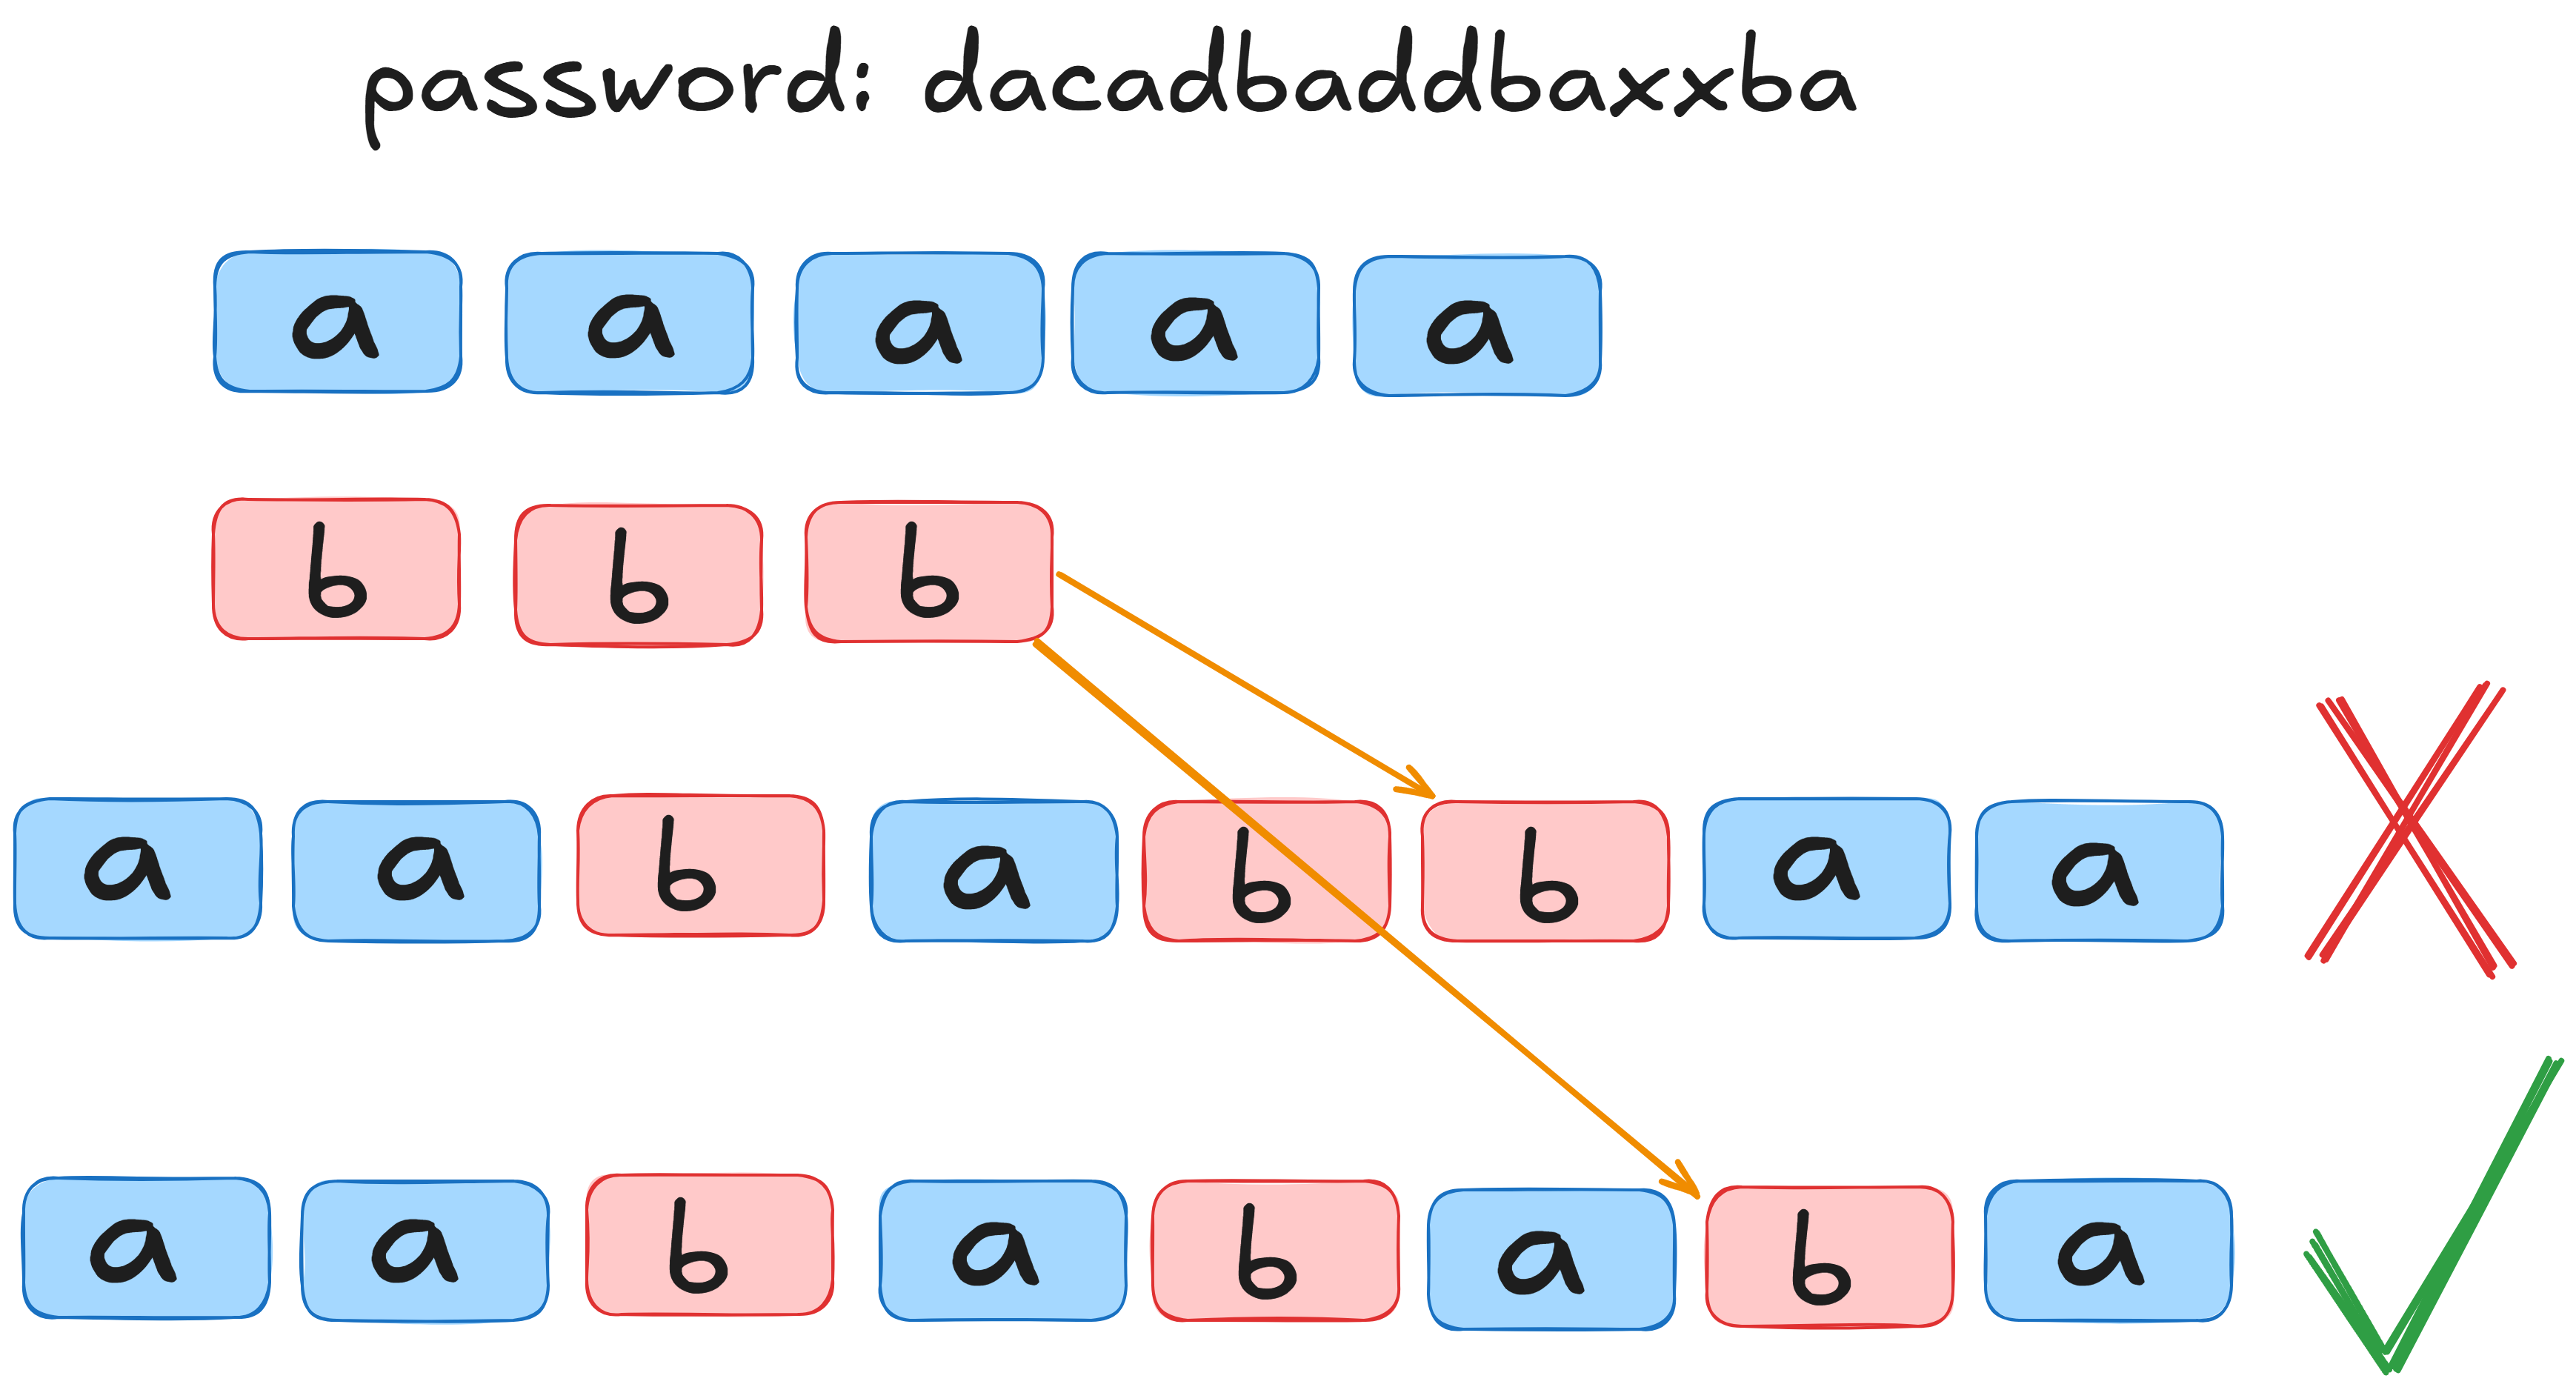
\includegraphics[width=0.8\linewidth]{img/select.png}
    \caption{Unión de dos secuencias en ''dacadbaddbaxxba"}
    \label{fig:enter-label}
\end{figure}

\end{bloque}
\end{frame}

\begin{frame}
\begin{bloque}[\textcolor{green}{password2} (\href{https://www.infoarena.ro/problema/password2}{infoarena})]

\textbf{Idea:} realizar $S$ consultas para cada letra, luego podemos unir de la siguiente forma:

\begin{itemize}
    \item Sean las secuencias $u_1, u_2, \dots, u_n$ y $v_1, v_2, ..., v_m$.
    \item Para cada $i$, desde $1$ hasta $n$, intentar colocar $u_i$ antes o después de los primeros $j$ de $v$, nota
    que tanto el índice $i$ (acierto) como el $j$ (fallo) aumenta, por tanto, se puede realizar en $n + m$ consultas.
    \item resolvemos con el algoritmo de Huffman Tree, por tanto, gastamos a lo más $S + N\log S$ consultas.
\end{itemize}

\end{bloque}
\end{frame}

\begin{frame}{Argumento Estructural y de Intercambio}
\begin{definicion}
\begin{itemize}
    \item {\bfseries Arg. Estructural}: Prueba que cualquier solución óptima debe tener cierta estructura. Ejm: Existe un Huffman Tree, tal que nodos con menor peso son hermanos.
    \item {\bfseries Arg. Intercambio}: Comparamos la solución del algoritmo con una óptima y muestra que cambiar partes mejora o no empeora.
\end{itemize}
\end{definicion}
\end{frame}

\begin{frame}
\begin{bloque}[\textcolor{black}{POI 2007 Weights} (\href{https://szkopul.edu.pl/problemset/problem/h_QPStxSmfEHuL2h_I5Qpa29/site/?key=statement}{szkopul})]

Se tienen $n$ contenedores con capacidades $c_1, c_2, \dots, c_n$ y $m$ pesas con masas $w_1, w_2, \dots, w_m$. Cada contenedor puede contener cualquier número de pesas, siempre que la suma de sus masas no exceda su capacidad. Además, para todo par $i, j$, se cumple que $w_i \mid w_j$ o $w_j \mid w_i$. Se desea encontrar la cantidad máxima de pesas que pueden colocarse respetando estas condiciones.

\end{bloque}
\end{frame}

\begin{frame}
\begin{bloque}[\textcolor{black}{POI 2007 Weights} (\href{https://szkopul.edu.pl/problemset/problem/h_QPStxSmfEHuL2h_I5Qpa29/site/?key=statement}{szkopul})]

\textbf{Idea:} 

\begin{itemize}
    \item Podemos usar \textbf{búsqueda binaria} sobre la cantidad de pesas a colocar -- probamos si es posible con los $k$ menores pesos --.
    \pause
    \item Sea $S$ un conjunto de pesas que puede ser colocado completamente en los contenedores sin exceder sus capacidades, y sea $m_{max}$ la masa de la pesa más pesada en $S$. Denotamos por $C_S$ el conjunto de todas las configuraciones válidas para $S$.
\end{itemize}
\end{bloque}
\end{frame}

\begin{frame}
\begin{bloque}[\textcolor{black}{POI 2007 Weights} (\href{https://szkopul.edu.pl/problemset/problem/h_QPStxSmfEHuL2h_I5Qpa29/site/?key=statement}{szkopul})]

\textbf{Idea:} 

\begin{itemize}
    \item \textbf{Argumento Estructural:} 
    Para cualquier contenedor $t$ con capacidad $w_t \geq m_{\max}$, existe una configuración válida $\mathcal{C}^* \in C(S)$ donde la pesa $m_{\max}$ está colocada en $t$.
\end{itemize}
\end{bloque}
\end{frame}

\begin{frame}
\begin{bloque}[\textcolor{black}{POI 2007 Weights} (\href{https://szkopul.edu.pl/problemset/problem/h_QPStxSmfEHuL2h_I5Qpa29/site/?key=statement}{szkopul})]

\textbf{Prueba:} 

Sea una configuración cualquiera y veamos que podemos colocar $m_{max}$ en $j$.   

\begin{itemize}
    \item Si la suma de pesos en el contenedor $j$ es menor o igual al máximo peso, los podemos intercambiar sin ningún problema. 
    \pause
    \item En otro caso, ordenamos el contenedor $j$, de mayor a menor $w^{'}_1, w^{'}_2, ..., w^{'}_m$, sea $k$ tal que \(\sum\limits_{i=1}^k w^{'}_i \le m_{max} < \sum\limits_{i=1}^{k+1} w^{'}_i\), se cumple $\sum\limits_{i=1}^k w^{'}_i = m_{max}$ 
\end{itemize}
\end{bloque}

\end{frame}

\begin{frame}
\begin{bloque}[\textcolor{black}{POI 2007 Weights} (\href{https://szkopul.edu.pl/problemset/problem/h_QPStxSmfEHuL2h_I5Qpa29/site/?key=statement}{szkopul})]

    
\textbf{hint:} Note que $w^{'}_1 \vert m_{max}$, y en general $w^{'}_{r + 1} \vert (m_{max} - \sum\limits_{i=1}^r w^{'}_i)$, para todo $r \le k$.
    
\end{bloque}

\end{frame}


\begin{frame}
\begin{bloque}[\textcolor{blue}{Coins} (Polish Junior Olympiad)]
Se te dan $n$ pilas de monedas. Cada pila contiene exactamente dos monedas. Conoces el valor de cada una de las $2n$ monedas. Puedes seleccionar como máximo $k$ monedas, con la siguiente restricción: 

\begin{itemize}
    \item \textbf{Si eliges la moneda inferior de una pila, también debes elegir la superior de esa misma pila.}
\end{itemize}

Determina el valor total máximo que puedes obtener al seleccionar las monedas

\end{bloque}
\end{frame}

\begin{frame}
\begin{bloque}[\textcolor{blue}{Coins} (Polish Junior Olympiad)]

\textbf{Idea:}
\begin{itemize}
    \item Hay dos tipos de pilas, las que tienen el máximo valor en la cima, y las que no.
    \pause
    \item \textbf{Argumento de intercambio:} Si solo hay pilas del tipo 1. Existe una solución óptima que respeta la condición de orden en la elección. (\textbf{hint:} Nunca es óptimo tomar la ficha de abajo antes que la de encima)
\end{itemize}

\end{bloque}
\end{frame}

\begin{frame}
\begin{bloque}[\textcolor{blue}{Coins} (Polish Junior Olympiad)]

\begin{itemize}
    \item \textbf{Argumento Estructural:} Si solo hay fichas del tipo 2. Existe una solución que solo toma a lo más una ficha de encima sin su ficha de abajo.\\
    \pause
    \textbf{Prueba:} Sean las pilas $p_1 = (a_1, b_1)$ y $p_2 = (a_2, b_2)$, tal que $a_1 < b_1$ y $a_2 < b_2$, sin perdida de generalidad $a_1 \le a_2$. Entonces

\[
    a_1 + a_2 ~(\text{tomar la cima de ambas}) < 
\]
\[
    a_2 + b_2 ~(\text{tomar solo una})
\]

    Dos pilas no pueden ser tomadas parcialmente.

\end{itemize}

\end{bloque}
\end{frame}

\begin{frame}
\begin{bloque}[\textcolor{blue}{Coins} (Polish Junior Olympiad)]

\begin{itemize}
    
    \item Si tomamos $k_1$ fichas de pilas de tipo 1, estas siempre pueden ser las $k_1$ fichas mayores, si tomamos $k_2$ fichas de pilas de tipos 2, si es una cantidad par, tomamos las $k_2 / 2$ pilas con valor total mayor, en otro caso tomamos la mayor ficha de cima no escogida, o tomamos la siguiente mayor pila y quitamos la menor fichar de abajo escogida.   
    
\end{itemize}

\end{bloque}
\end{frame}

\begin{frame}
\begin{bloque}[\textcolor{blue}{Coins} (Polish Junior Olympiad) ]

\begin{figure}
    \centering
    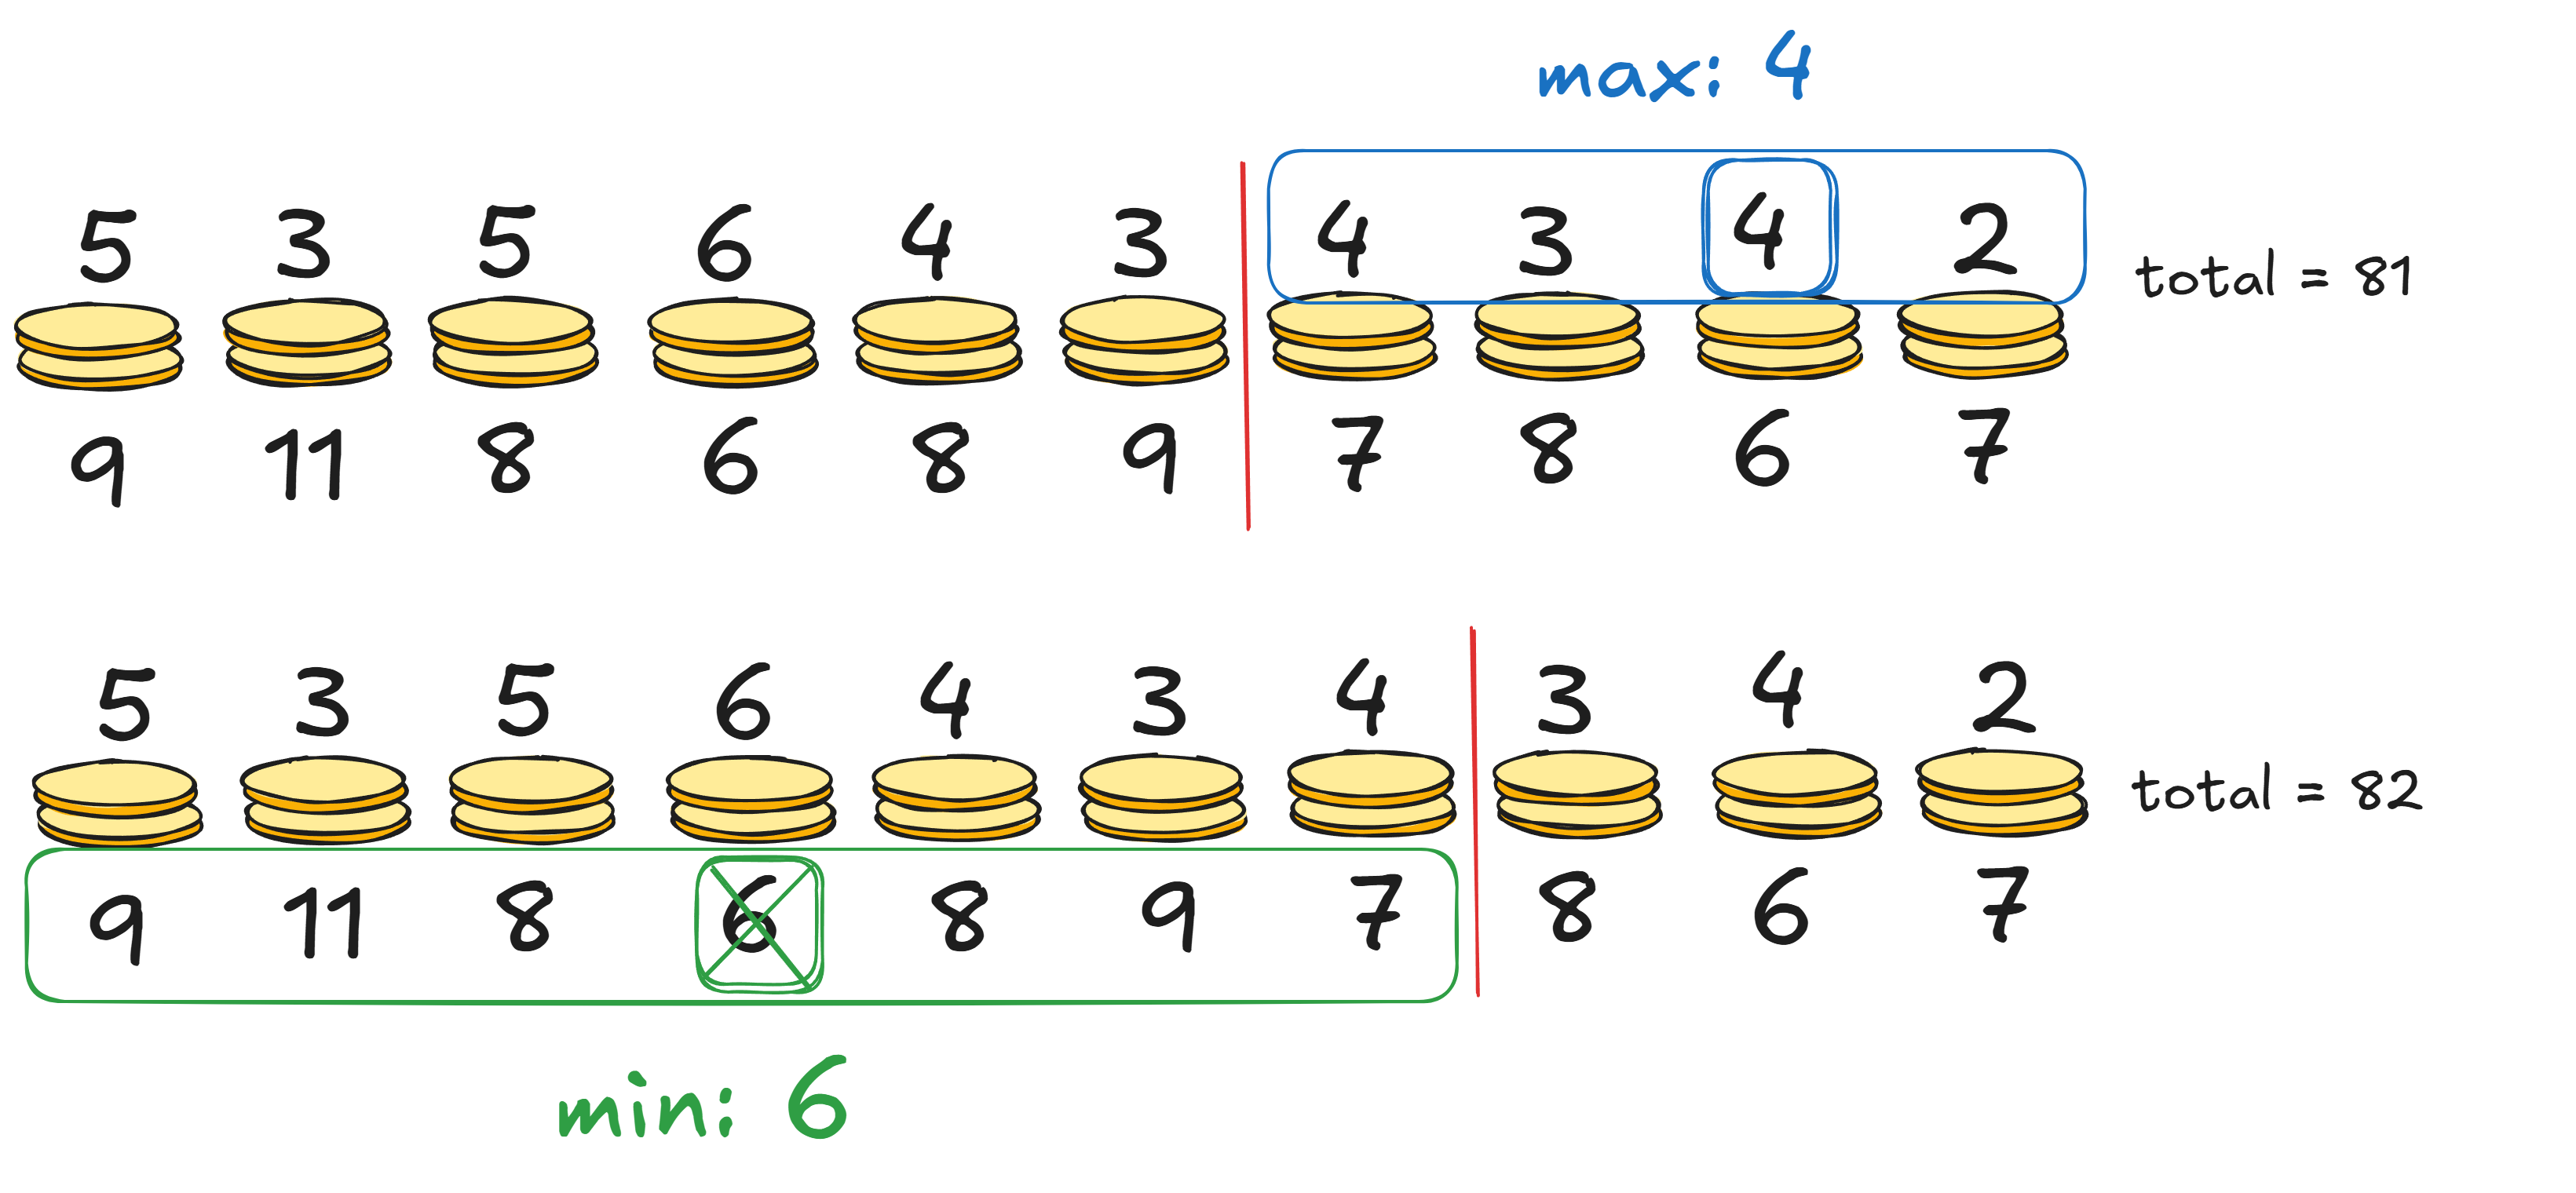
\includegraphics[width=0.97\linewidth]{img/coins-greedy.png}
    \caption{Elección de $k=7$ fichas de pilas del tipo 2.}
    \label{fig:enter-label}
\end{figure}

\end{bloque}
\end{frame}

\begin{frame}

\centering
\Large Gracias.

\end{frame}
\end{document}